\section{Analyse semantique}
L'analyse sémantique consiste à verifier l'exactitude des types, des
    déclarations,... . Elle a pour but de verifier le sens de la phrase ecrite.
    
    \begin{figure}[h]
        \begin{lstlisting}[style=base]
            si Vrai == 0 alors
                Vrai + 1
            fin si \end{lstlisting}
        Cette phrase est syntaxiquement juste mais sémentiquement fausse
    \end{figure}
    
Pour palier a ce problème on va mettre un place un système d'attribut, qui
donnera un sens, une valeur aux outils de la grammaire avec lesquels nous
avons réalisé l'analyse syntaxique ce sens sera definis par les attributs.

\subsection{Les attributs}
    L'analyse sémantique repose sur un principe : 
	Un attribut est une valeur quantifiée associée à un
    élément du langage. L'élément peut être n'importe quoi, un type d'expression
    , une valeur, etc etc . Chaque élément du langage est représenté par un
    symbole 
    auquel l'attribut sera associé. on note alors, A.a ou a est l'attribut de 
    l'élément A. Le calcule de ces attributs se fait en fonction de la
    grammaire utilisée dans l'analyse syntaxique on associes donc à chaque
    aspects de la grammaire des règles sémentiques. cette grammaire est alors
    dites attribuée et l'arbre syntaxique qui porte alors en chacun de ses
    noeud la valeurs des attributs du même noeud sera appelés arbre syntaxique
    décoré. Il existe deux types d'attributs.

\subsubsection{Attributs synthétisé}
	Un attributs synthétisé se calcule au niveau d'un noeud A en fonction de la valeur d'attribut de ses fils \\
	
\ovalbox{
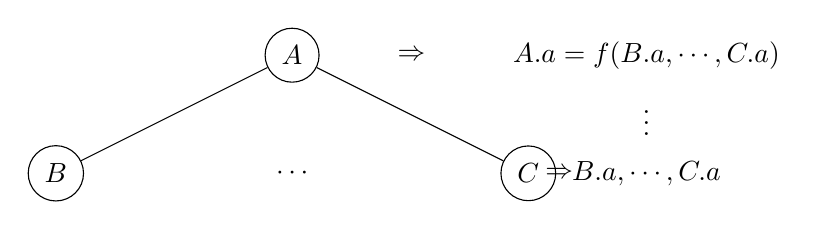
\begin{tikzpicture}[level/.style={sibling distance=60mm/#1}]
\node [circle,draw] (z){$A$}
  child {node [circle,draw] (a) {$B$}
      } 
  child {node [circle,draw] (b) {$C$}
  child [grow=right]{node  (e) {$B.a,  \cdots, C.a$} edge from parent[draw=none]
    child [grow=up]  {node (c) {$A.a = f(B.a, \cdots, C.a) $} edge from parent[draw=none]
  }
  }
  };
\path (a) -- (b) node (f) [midway] {$\cdots$};

\path (b) -- (e) node [midway] {$\Rightarrow$};
\path (z) -- (c) node [midway] {$\Rightarrow$};
\path (e) -- (c) node [midway] {$\vdots$};
\end{tikzpicture}}

Il s'agit donc d'un analyse ascendante.

\subsubsection{Attributs hérités}
 Ces attributs sont un peu l'inverse des attributs synthétisés car ils ne sont
 pas calculé a l'aide des fils mais à l'aide des noeuds parents et des noeuds
 frères. Cette analyse est qualifié de descendante et permet de situé chaque
 noeud dans un contexte.
\\
 Une fois ces calculs effectués notre analyse va pouvoir verifier si la phrase a
 un sens en fonction des attributs calculés. Si le resultats en tout noeud de
 notre arbre est logique (reviens basiquement a dire que 1+1 = 2) alors notre
 sémantique et respecter et nous pouvons passer a la génération de code.

\subsection{Ouverture de l'analyse sémantique}
    L'analyse sémantique peut devenir vraiment complexe si l'on decide de
    traiter plusieurs sources et plusieurs destinations. C'est a ce moment
    qu'intervient les schemas de compilation qui permettront de definir
    plusieurs analyses differente mais pour le moment nous resterons uniquement
    sur une compilation d'une source vers une destination. 
